\documentclass{article}
\usepackage[T1]{fontenc}
\usepackage{lmodern}
\usepackage{graphicx}
\usepackage{amsmath,amssymb}
\usepackage[a4paper,margin=2cm]{geometry}
\usepackage[absolute,overlay]{textpos}
\setlength{\TPHorizModule}{1mm}
\setlength{\TPVertModule}{1mm}
\usepackage[indonesian]{babel}
\usepackage{hyperref}
\setlength{\emergencystretch}{2em}
% unit: Halaman 71

\begin{document}

% === Halaman 71 (llm) ===

\vspace{240.57mm}

\textbf{Gambar} pembangkitan kunci putaran di dalam DES

% deskripsi: Diagram alir proses pembangkitan kunci putaran (key scheduling) dalam algoritma DES, menunjukkan transformasi dari Kunci eksternal 64 bit melalui Permutasi PC-1, pemisahan menjadi C dan D masing-masing 28 bit, operasi Left Shift berulang, dan Permutasi PC-2 untuk menghasilkan kunci sub-kunci $K_1, K_j,$ hingga $K_{16}$ yang masing-masing berukuran 48 bit.
% bbox normalisasi: [0.0400, 0.1500, 0.6500, 0.9600]
\begin{textblock*}{128.10mm}(8.40mm,44.55mm)
\noindent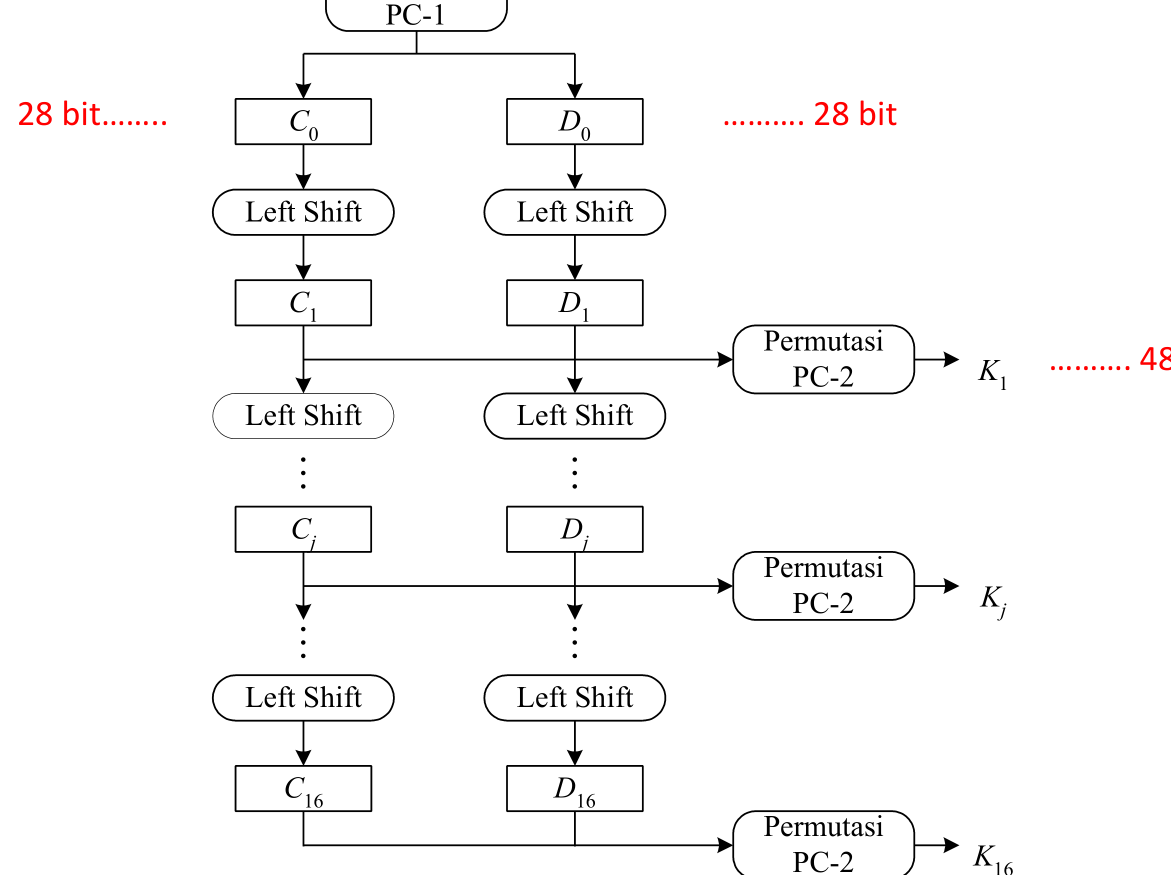
\includegraphics[width=128.10mm,height=240.57mm]{../../images/llm/page_071_img_01.png}%
\end{textblock*}

\end{document}
